GEANT4 is a free toolkit for the simulation of particles as they travel through matter\cite{agostinelli_geant4simulation_2003}.
In general two types of applications were authored with the GEANT4 toolkit; ranges along with energy deposition and light transport.
All of the applications shared a common electromagnetic physics list based on the Livermore data set, and a cross section driven hadron physics list was used for the neutron interactions.
Ions were transported with the general ion physics list which contains detailed alpha and triton models.
Optical photons were transported with the default Optical Photon physics list.
More details on the GEANT4 toolkit may be found in \autoref{chap:G4Intro}.

\subsection{Energy Deposition Simulations}
\label{sec:EnergyDeposition}
The GEANT4 toolkit has the ability to track the energy deposition in different materials as well as the tracking of electrons to a least \SI{1}{\keV}\cite{agostinelli_geant4simulation_2003}.
It is proposed to represent the detector geometry as a single layer of neutron absorbing thin polymeric film mounted on top of a non-scintillating material (PMMA).
For simplicity, the initial events for runs will be chosen by setting up a particle gun for thermal (\SI{0.025}{\eV}) neutrons upon the detector and for both gammas resulting from a \iso[60]{Co} decay.
\begin{figure}
  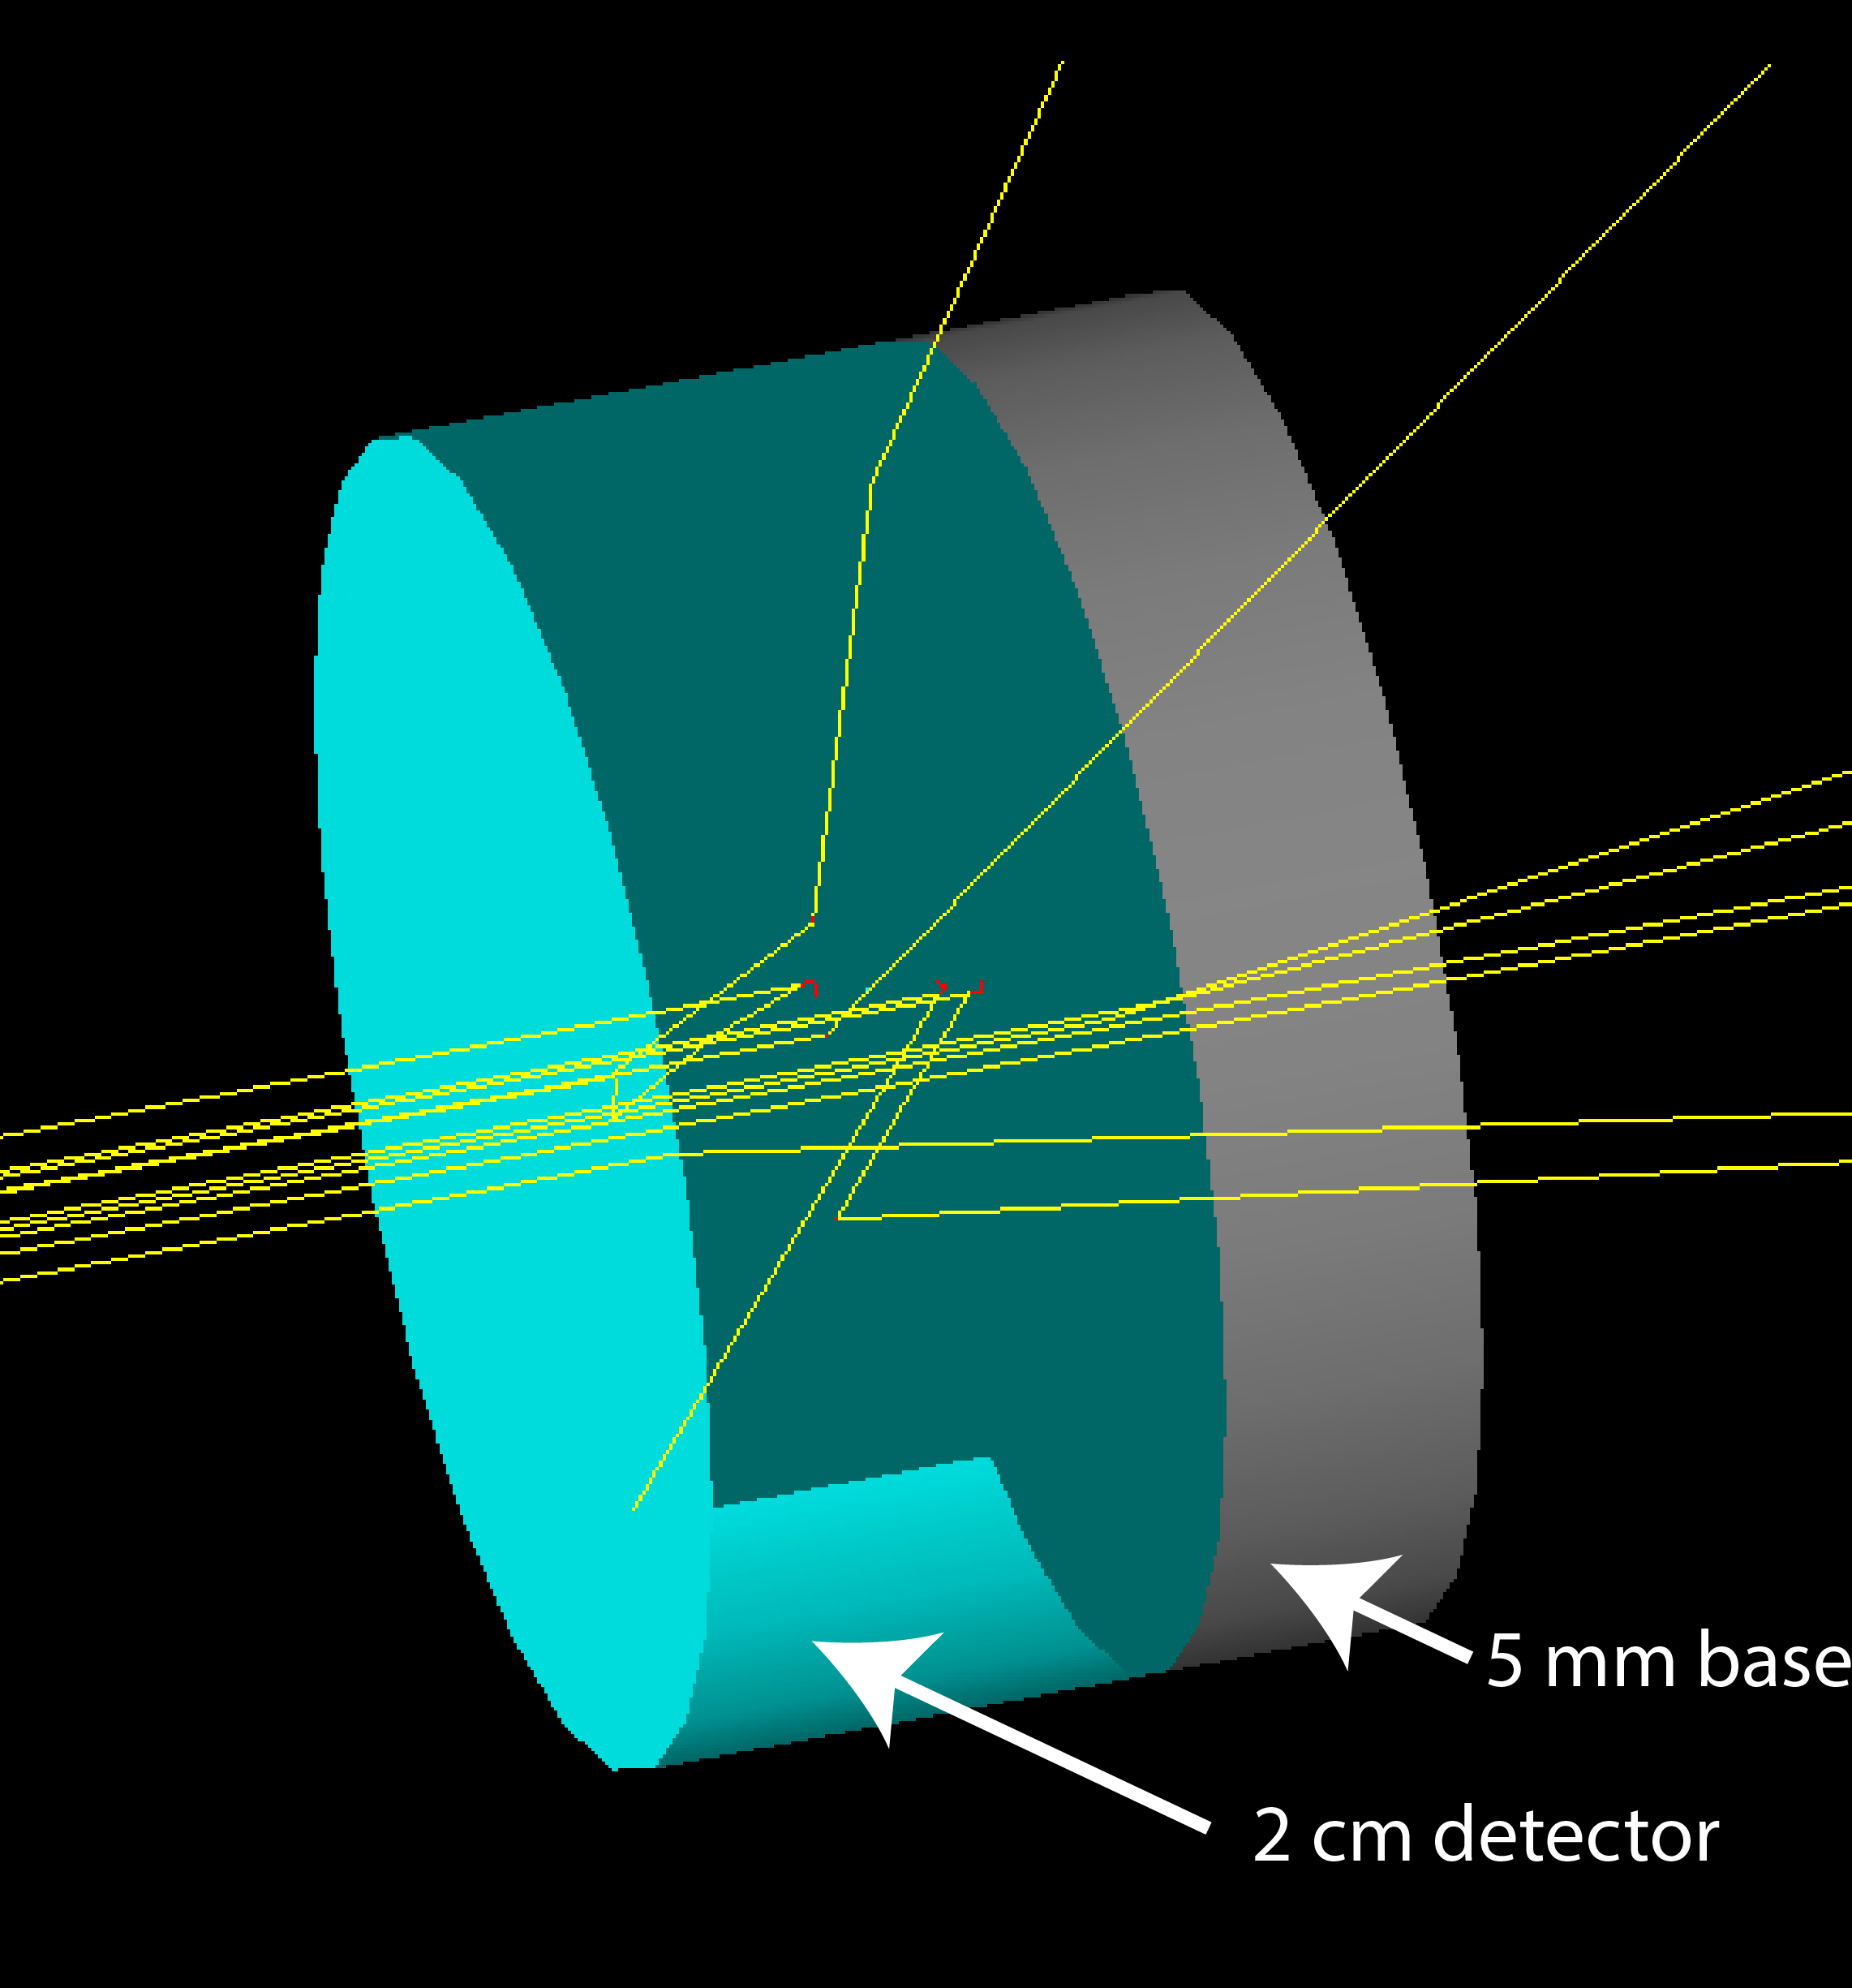
\includegraphics[width=\textwidth]{GEANT4AnnotatedGeo_EnergyDepEvent}
	\caption[GEANT4 Energy Deposition Geometry]{GEANT4 Geometry for the Simulation of Energy Deposition. What is shown are 10 photons from a \iso[60]{Co} source impingement upon a \SI{2}{\cm} thick detector.  The photon tracks are shown in yellow, while the electron tracks are shown in red.}
	\label{fig:EDepSimGeo}
\end{figure}
It is expected that the the Livermore data-driven parameterized electromagnetic physics will be necessary to calculate the ionizing energy deposition, extending the standard electro-magnetic physics down to \SI{1}{\kilo\eV}.
The neutron interactions will be simulated with a hadronic modules, using the \verb+HP+ flavored modules to use the ENDF cross sections to calculate the interaction rates.

\subsubsection{Energy Deposition Validation}
The validation of this GEANT4 simulation was completed by reproducing the single collision energy loss in water as well as comparing  the spectral shapes and averages of simulated and measured spectra.
The reproduction of the single collision energy loss will ensure that the electron physics are implemented correctly, while the simulation of the polymeric film energy deposition allows the user to gain confidence that the correct tracking and binning analysis has been implemented.

The simulation was validated by reproducing the single collision energy loss for water as well as comparing spectra shapes and averages of simulated spectra to the measured spectra.
The single collision energy loss spectra for water that was simulated is shown in \autoref{fig:SingleCollisionELossWater}.
In general there was excellent agreement between the simulated energy spectra and a previously published spectra\cite{turner_comparative_1982}, with the simulated spectra having much better resolution than the reference did not.
It is thought that this is due to the water model in GEANT4 having better cross sections than the previously published spectra.
\begin{figure}[ht]
  \centering
  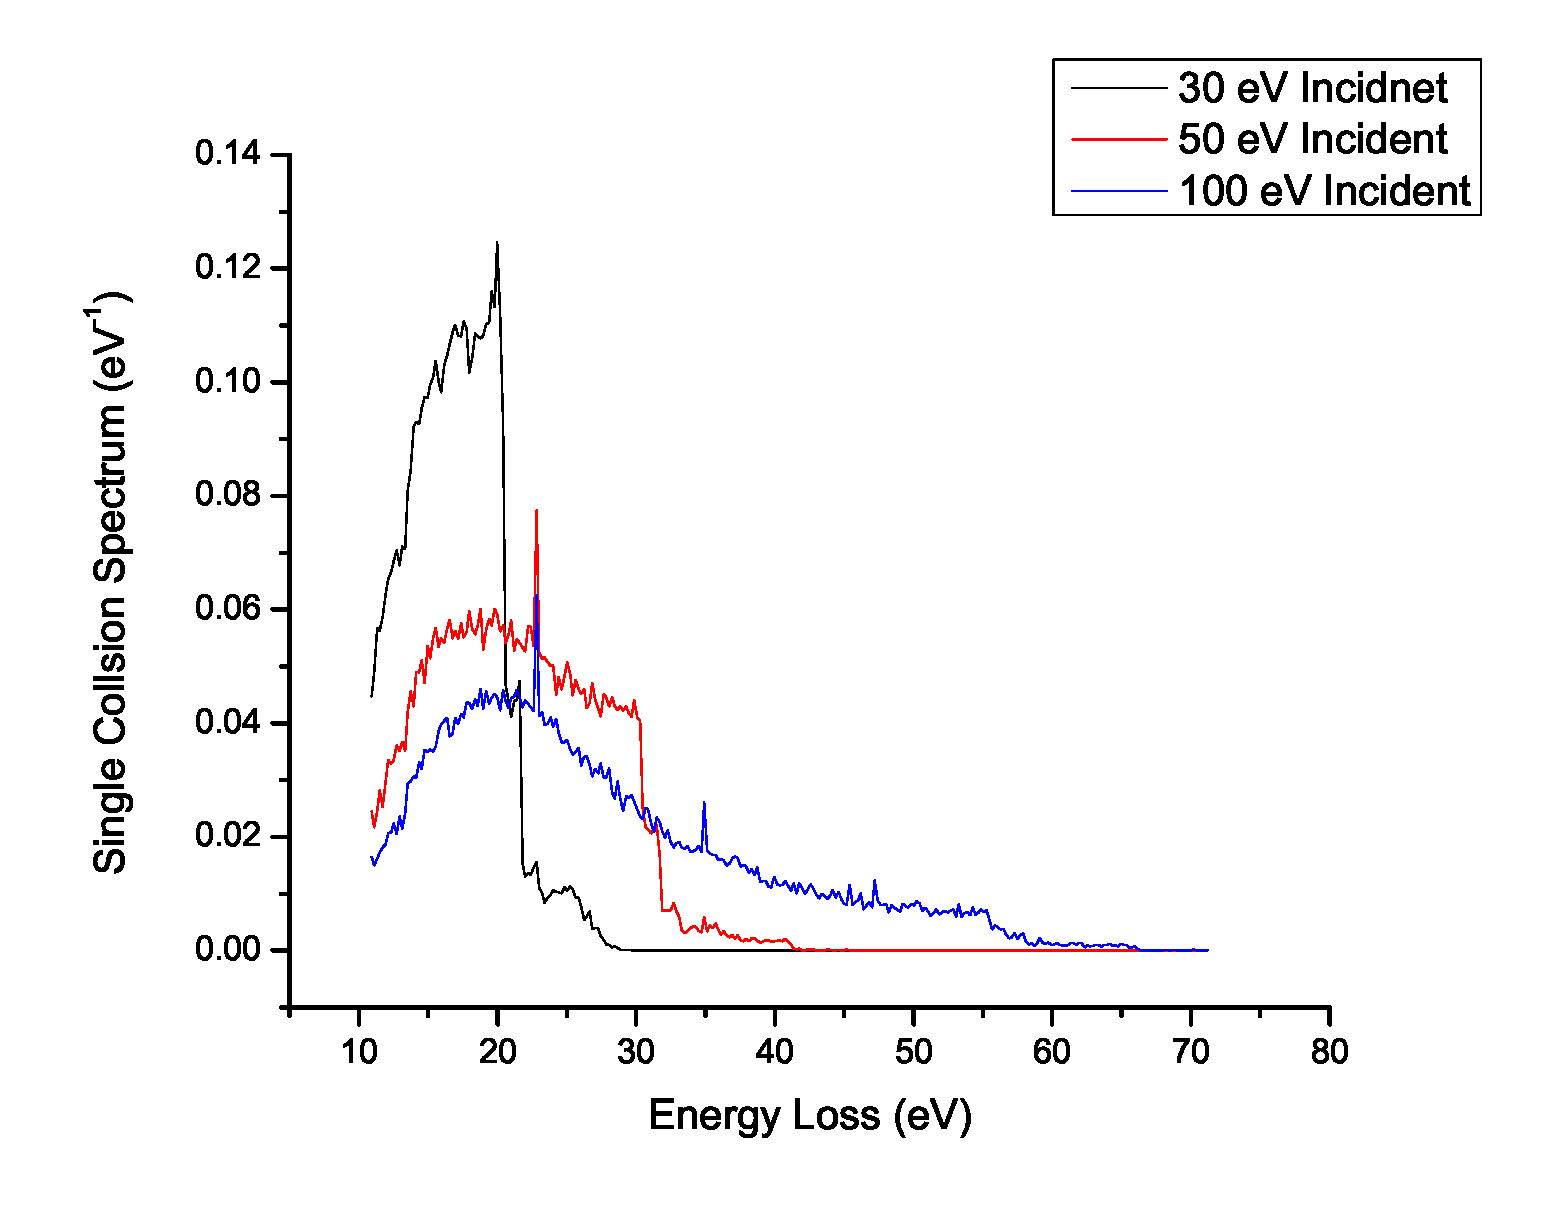
\includegraphics[width=\textwidth]{SingleCollisionEnergyLoss_300bins}
  \caption{Single Collision Energy Loss of Water. The simulated energy spectra matches that of Turner\cite{turner_comparative_1982}.}
	\label{fig:SingleCollisionELossWater}
\end{figure}

The validity of the GEANT4 simulation is determined by comparing the spectra shapes of measured spectra to simulated energy deposition.
Figure \ref{fig:spectraComparisonGamma} shows the comparison between the simulated energy deposition per incident photon from a \iso[60]{Co} source and the measured pulse height spectra from the \iso[60]{Co} irradiator per incident photon.
The energy calibration on the upper axis of the measured spectra was completed by finding the channel number at a given intrinsic efficiency and the corresponding energy at that intrinsic efficiency.
The energy of this feature on the measured spectra was then compared to the energy on the simulated spectra, with all of the values being within 10\%.
\begin{figure*}[ht]
	\centering
	\begin{subfigure}[b]{0.45\textwidth}
    		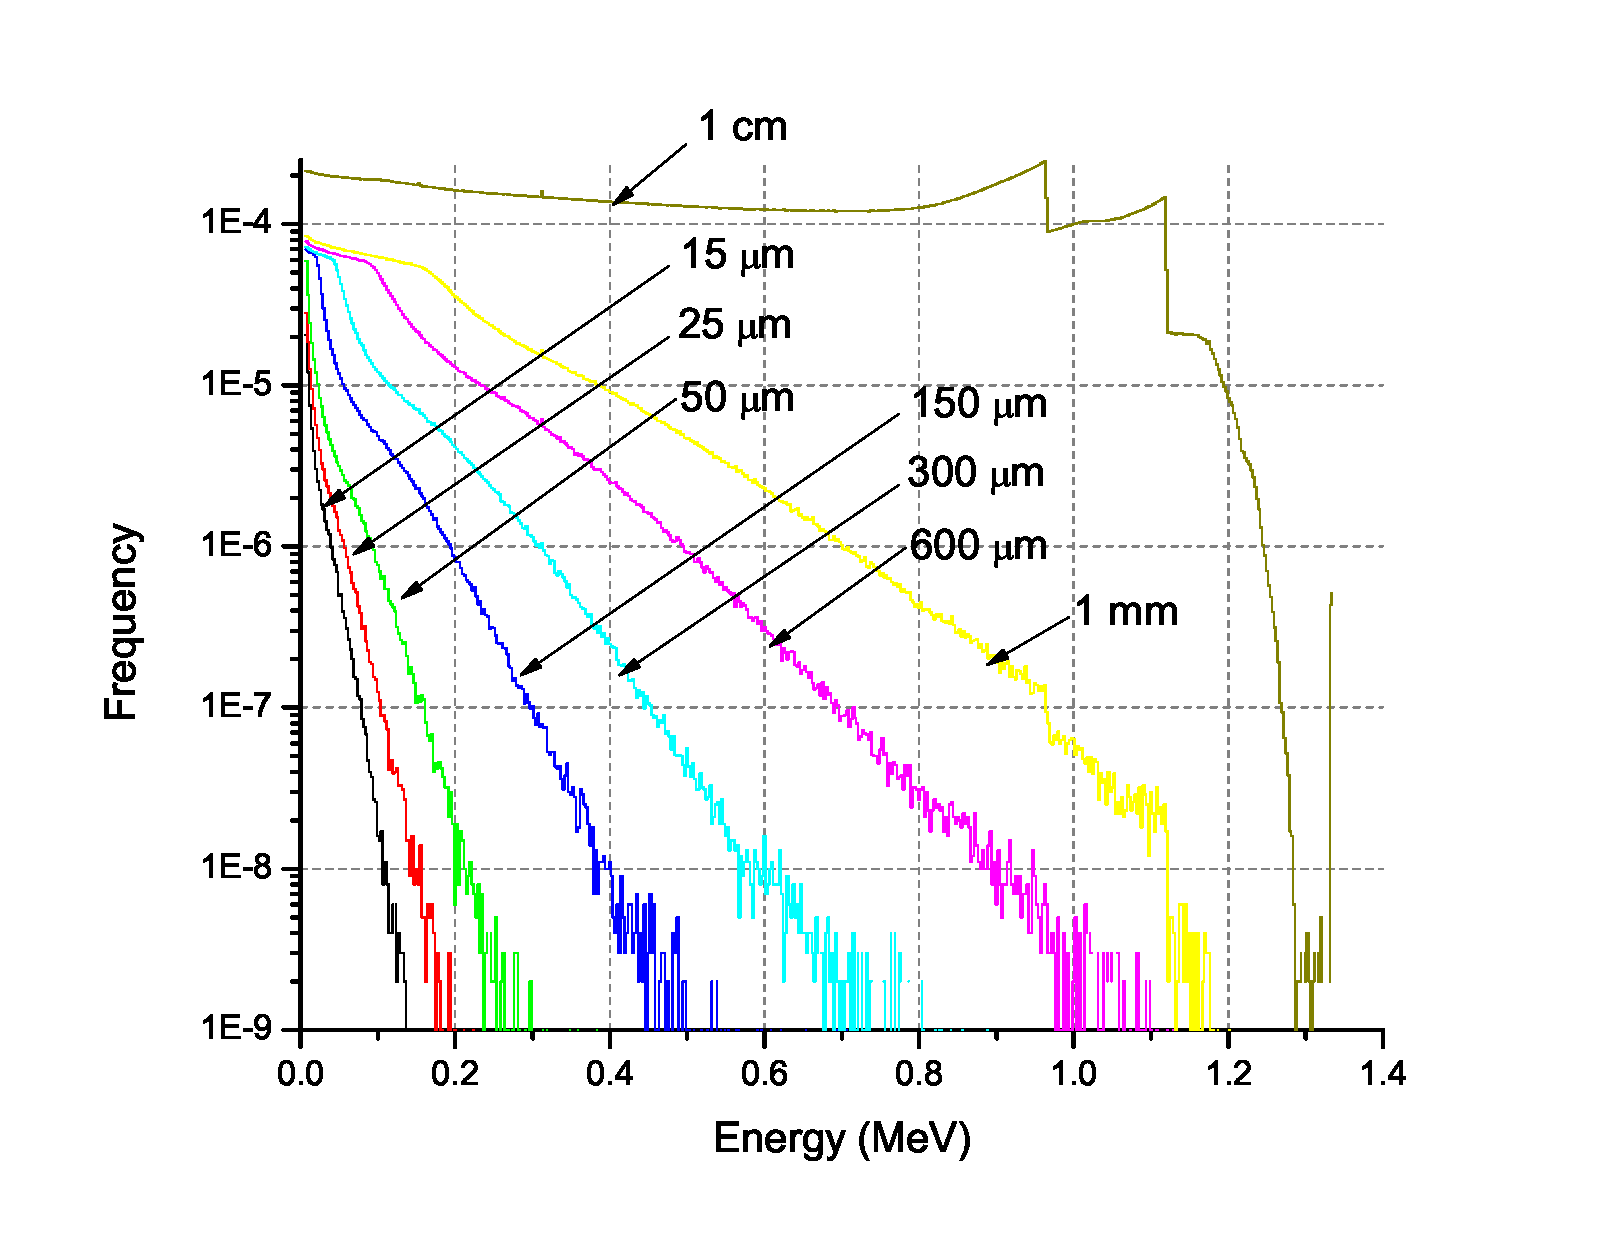
\includegraphics[width=\textwidth]{PS_EDepSim_Co60}
		\caption{GEANT4 Simulated Energy Deposition}
	\end{subfigure}%
	~
	\begin{subfigure}[b]{0.45\textwidth}
    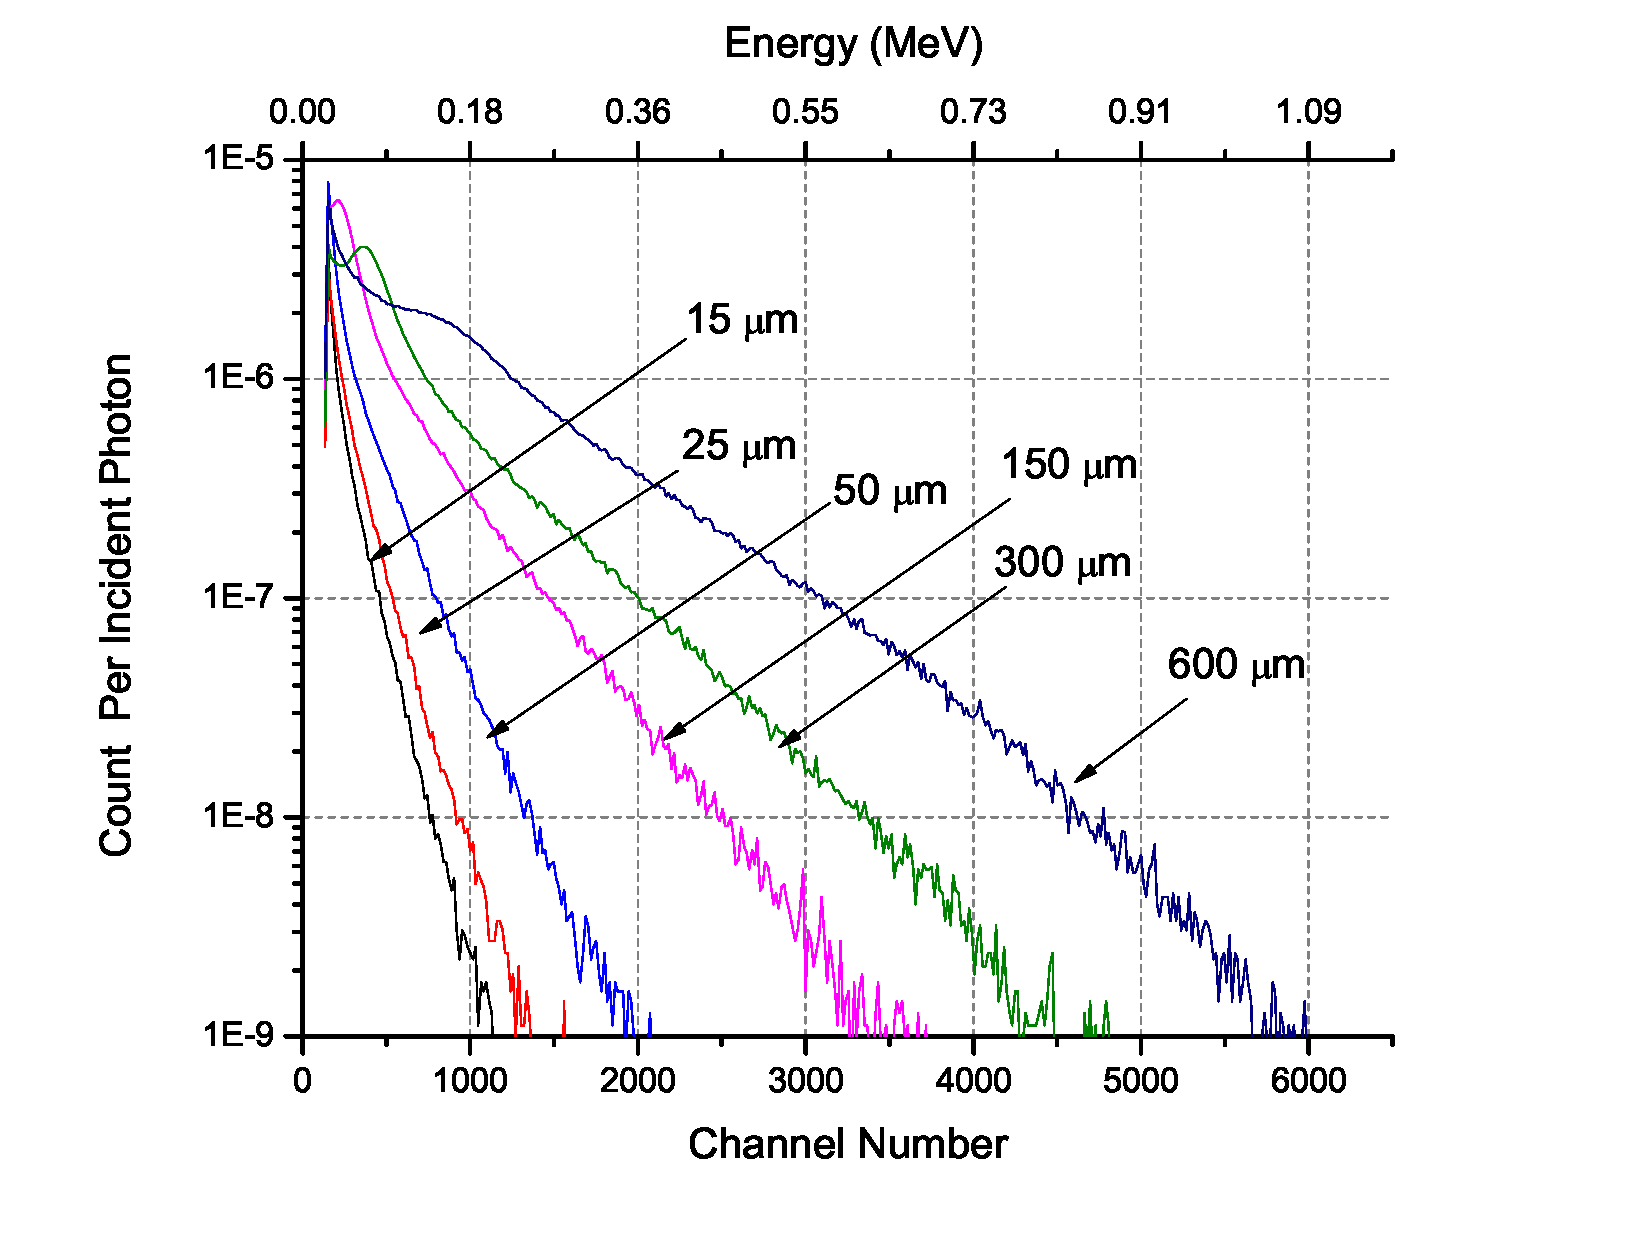
\includegraphics[width=\textwidth]{PS_GammaCR-Binned-FluxNorm_20LiF_5PPO}
		\caption{Measured Pulse Height Spectra}
	\end{subfigure}%
	\caption{Comparison of the energy deposition and binned pulse height spectra for validation. The spectra have the same shape, indicating agreement. The fabricated films greater than \SI{600}{\um} were of poor optical quality and therefore their results are not shown.}
	\label{fig:spectraComparisonGamma}
\end{figure*}
The average energy deposition and average pulse height are shown in Figure \ref{fig:EDepLightYield}. 
With the average energy deposition on the left axis and the average light yield (pulse height) on the right axis, it is possible to compare the measurement and the simulation and agreement is observed.
\begin{figure*}[ht]
	\centering
	\begin{subfigure}[b]{0.45\textwidth}
    		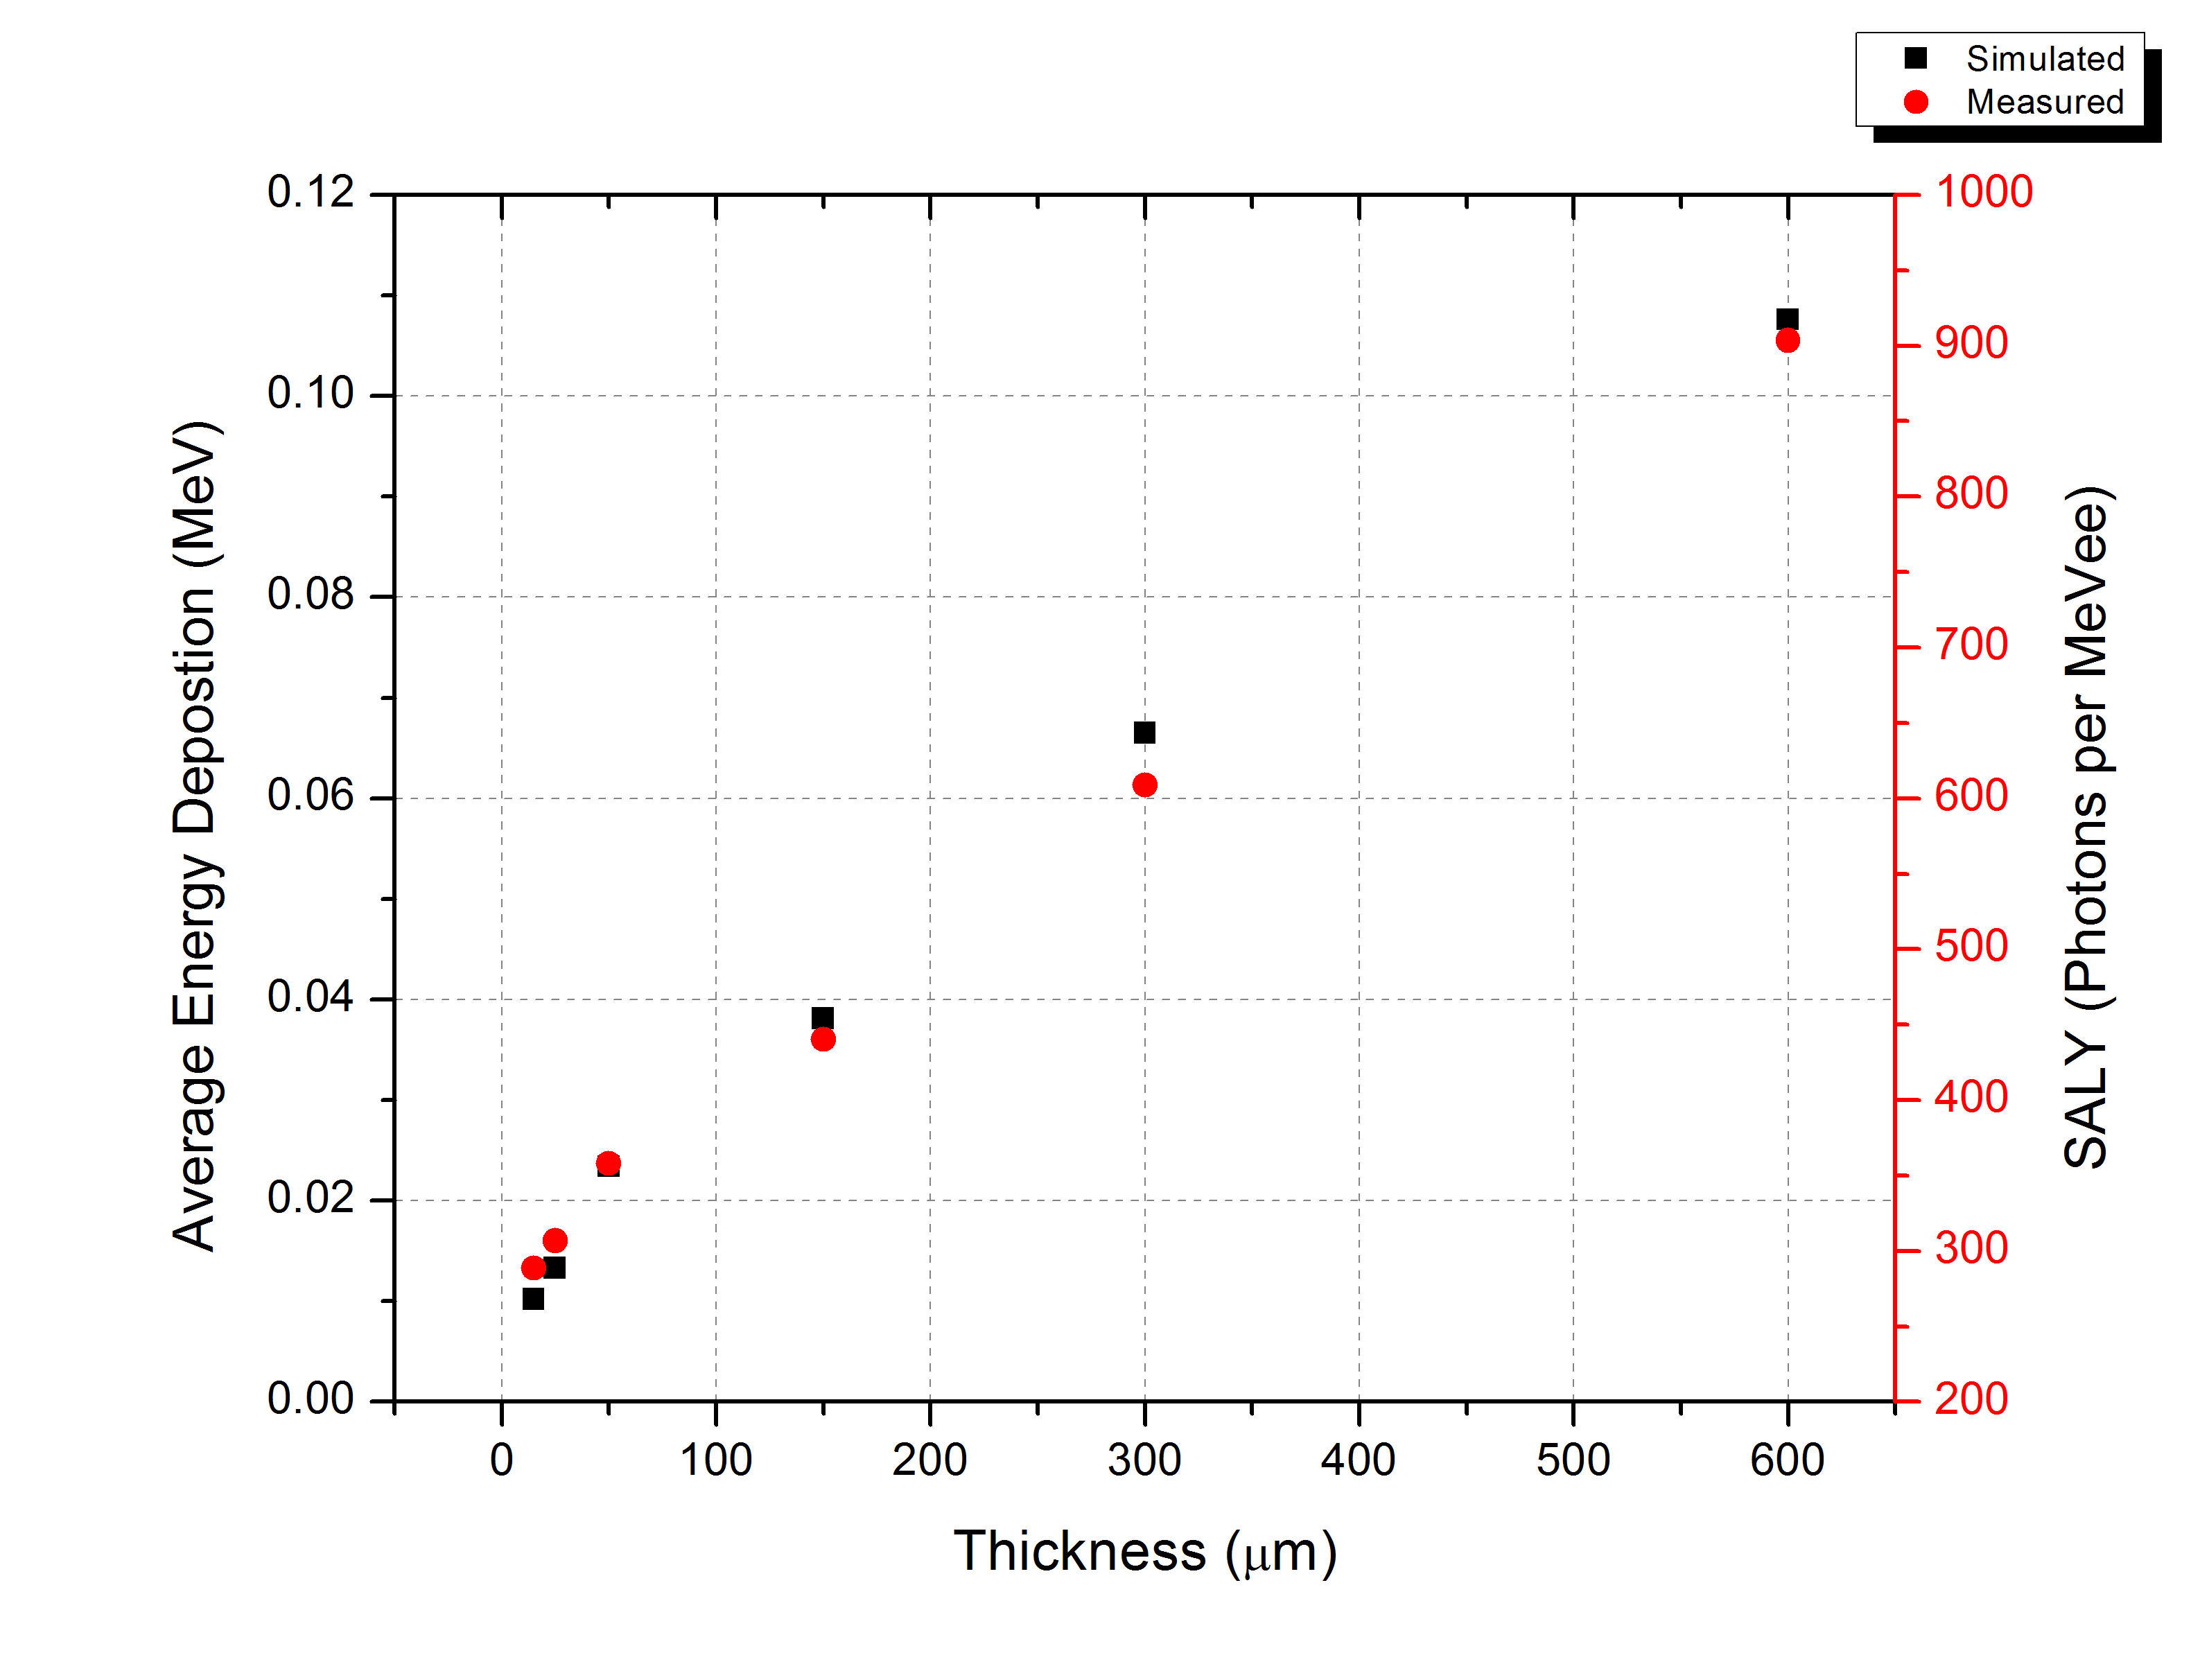
\includegraphics[width=\textwidth]{G4EDep_LightYield_Co60}
		\caption{Gamma (\iso[60]{Co})}
	\end{subfigure}%
	~
	\begin{subfigure}[b]{0.45\textwidth}
    		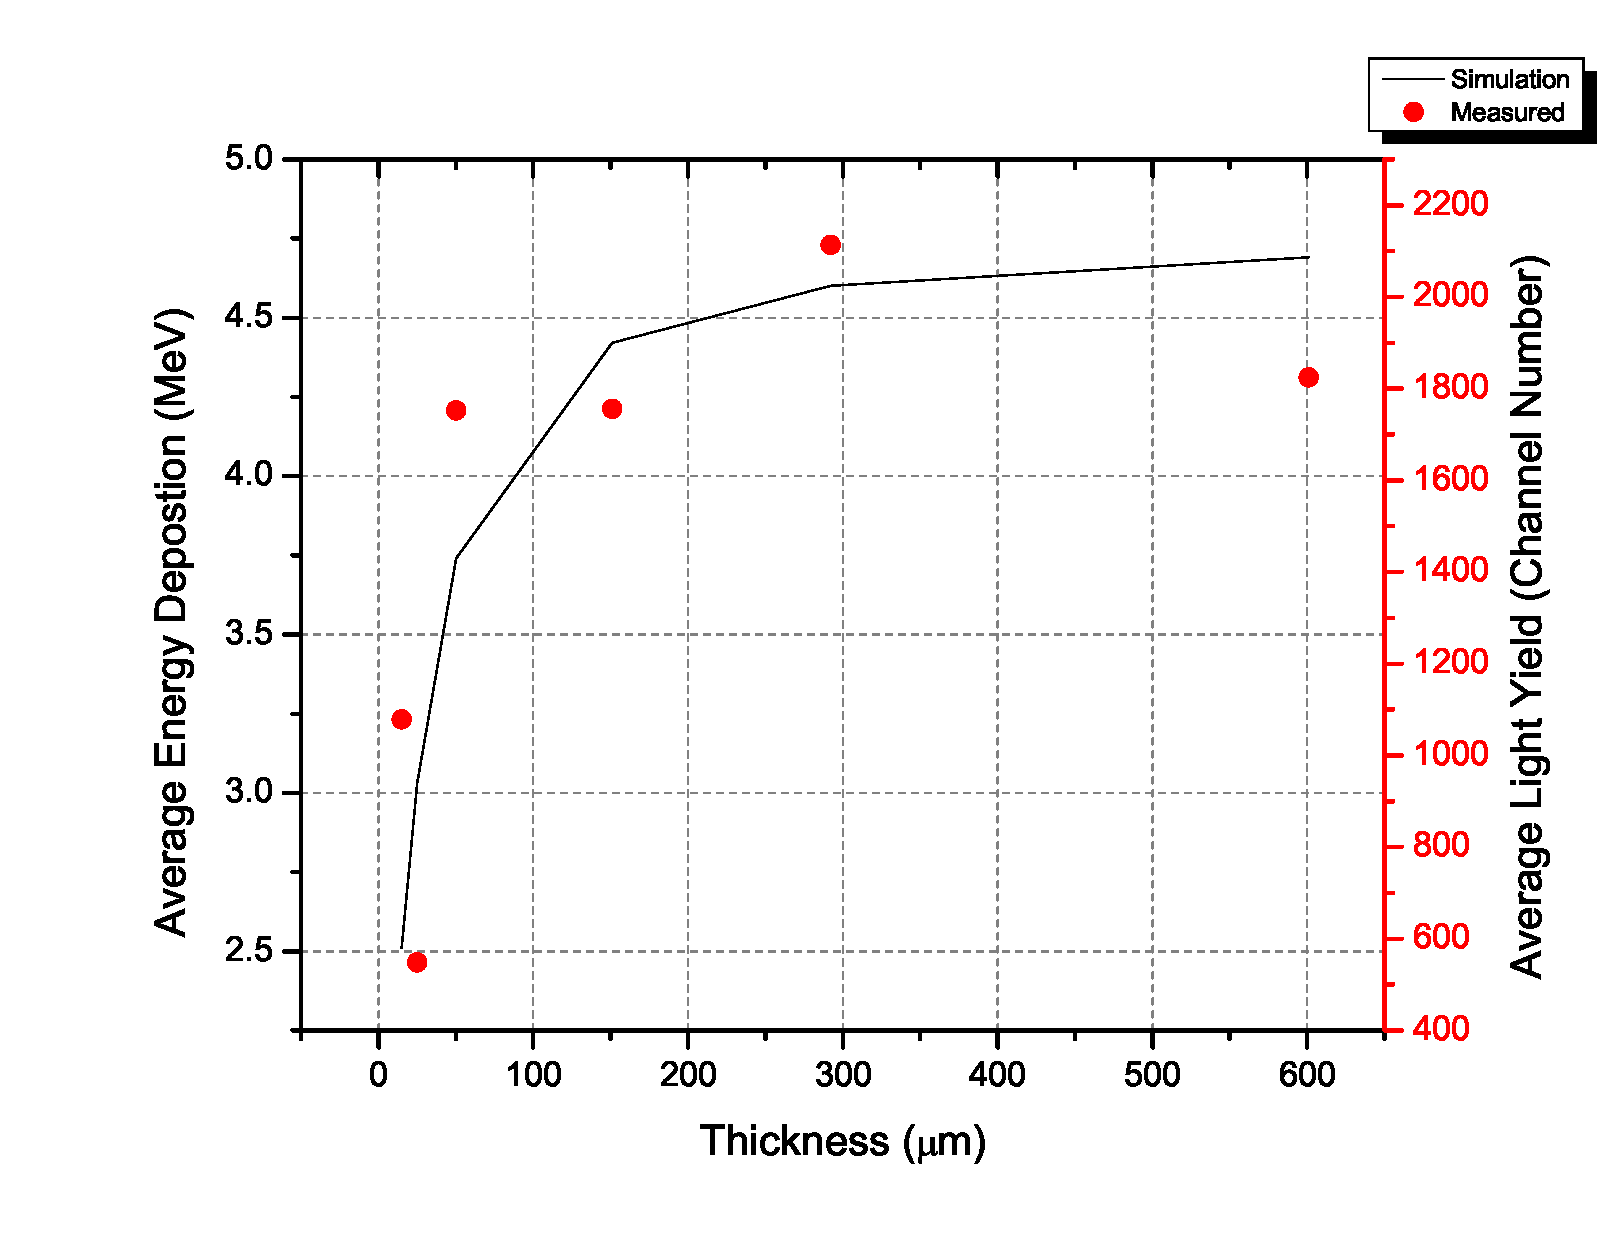
\includegraphics[width=\textwidth]{G4EDep_LightYield_Neutron}
		\caption{Neutrons}
	\end{subfigure}%
	\caption{Average Energy Deposition and Measured Light Yield. The solid lines are calculated values and the red dots are measurements.}
	\label{fig:EDepLightYield}
\end{figure*}

\subsection{Optical Photon Simulatioins}
\label{sec:OpticalPhotonSims}
Photons are considered to be optical photons in the GEANT4 model when the wavelength of the photon is much greater than atomic spacing to allow for their wave-like nature.
The processes for optical photons included in GEANT4 are  refraction and reflection at 
\autoref[tab:G4OpticalParameters} provides a summary of the different optical parameters available in the GEANT4 model.
\begin{table}
	\caption[Optical Parameters Available in GEANT4]{Optical Parameters Available in the GEANT4 model}
	\label{tab:G4OpticalParameters}
	\begin{tabular}{p{2cm} | m{5cm}
	\toprule
	Category & Parameter \\
	\midrule
	General & RINDEX, ABSLENGTH \\
	Scintillation & SCINTILLATION, FASTCOMPONENT, SLOWCOMPONENT, SCINTILLATIONYIELD, RESOLUTIONSCALE, FASTTIMECONSTANT, SLOWTIMECONSTANT, YIELDRATIO \\
	WLS & WLSABSLENGTH, WLSCOMPONENT, WLSTIME \\
	Boundary & Finish, Model, Type, RINDEX, SPECULARLOBECONSTANT, BACKSCATTERCONSTANT, REFLECTIVITY, EFFICIENCY, POLISH \\
	\bottomrule	
	\end{tabular}
\end{table}
Optical photons were simulated in GEANT4 by creating an optical material property for each of the optical materials.
In general this involves setting the scintillation yield of the material, the resolution of the material, the optical photon absorbance of the film and the decay time.
It is also possible to set the Birks parameter of the material to simulate the light quenching of the material.
The Birks parameter for the materials were found by varying the 
\autoref{tab:G4LightSimParam} enumerates several of the parameters used in the simulations.
\begin{table}
	\caption[GEANT4 Material Scintillation Parameters]{Parameters used in the simulation of optical process in GEANT4}
	\label{tab:G4LightSimParm}
	\begin{tabular}{c | c}
	\toprule
	Parameter & Value \\
	\midrule
	Birks Parameter &  \cite{Tretyak_2010} \\
	\bottomrule
	\end{tabular}
\end{table}
 and 

